\documentclass[10pt, conference, letterpaper]{IEEEtran}
\usepackage{cite}
\usepackage{xcolor,soul,framed}
\usepackage{amsmath,amsthm,amssymb,amsfonts}
\usepackage{algorithmic}
\usepackage{graphicx}
\usepackage{color, soul}
\usepackage{algorithm, algorithmic}
\usepackage[utf8]{inputenc}
\usepackage[english]{babel}
\usepackage{mathtools}
\graphicspath{ {./images/} }

%---------------------------------------------------------------%
\newtheorem{definition}{Denifition}
\newtheorem{assumption}{Assumption}
\newtheorem{problem}{Problem}
\newtheorem{lemma}{Lemma}
\newtheorem{remark}{Remark}
\newtheorem{theorem}{Theorem}
\newtheorem{corollary}{Corollary}
\newtheorem{example}{Example}
\newcommand{\eq}{=}
\newcommand{\domZ}{\mathbb{Z}_{*}}
\newcommand{\vecOne}{\mathbf{1}}
\newcommand{\ind}{\mathbf{I}}
\newcommand{\mat}{\mathbf}
\newcommand{\define}{\triangleq}
\newcommand{\leadto}{\Rightarrow}
\renewcommand{\vec}{\mathbf}
\DeclarePairedDelimiter{\set}{\{}{\}}
\DeclarePairedDelimiter{\norm}{|}{|}
\DeclarePairedDelimiter{\Inorm}{\|}{\|_1}
\DeclarePairedDelimiter{\Paren}{\bigg(}{\bigg)}
\DeclarePairedDelimiter{\Bracket}{\bigg[}{\bigg]}
\DeclarePairedDelimiter{\Brace}{\bigg\{}{\bigg\}}
%---------------------------------------------------------------%
\newcommand{\apSet}{\mathcal{K}}
\newcommand{\esSet}{\mathcal{M}}
\newcommand{\jSpace}{\mathcal{J}}
\newcommand{\wSet}{\mathcal{W}}
\newcommand{\uSet}{\mathcal{U}}
\newcommand{\cSet}{\mathcal{C}}
\newcommand{\Stat}{\mathbf{S}}
\newcommand{\Obsv}{\mathcal{Y}}
\newcommand{\Policy}{\mathbf{\Omega}}
%---------------------------------------------------------------%

\begin{document}

    %=============================== TITLE ===============================%
    \title{
        Meet-in-Future: Distributed Online Job Dispatching with Obsolete Information in Edge Computing System
    }
    \author{
        \IEEEauthorblockN{
            Yuncong Hong\IEEEauthorrefmark{1}\IEEEauthorrefmark{2},
            % Rui Wang\IEEEauthorrefmark{1},
            % Haisheng Tan\IEEEauthorrefmark{3},
            % Francis C.M. Lau\IEEEauthorrefmark{2}
        }
        \IEEEauthorblockA{
            \IEEEauthorrefmark{1}Southern University of Science and Technology, P.R. China,
            \IEEEauthorrefmark{2}The University of Hong Kong, Hong Kong,\\
            \IEEEauthorrefmark{3}University of Science and Technology of China, P.R. China
        }
    }
    \maketitle

    %============================== ABSTRACT ==============================%
    \begin{abstract}
        \label{sec:abstract}
        Edge computing is believed to be the solid solution for time-sensitive big data real-time calculation. The cooperation among edge servers in the same coalition usually causes ineffective task scheduling due to obsolete information sharing, which is hard to tackle even with extra centralized agent design. In this work, we formulate the problem with job dispatching in distributed Edge Computing system, and identify the difficulty exists in cooperation between AP nodes (Access Points) and ES nodes (Edge Servers) with delayed information. We design the broadcast information in the system and formulate the corresponding problem into a MDP problem. The value function approximation and \st{one-step policy iteration method is adopted to obtain a sub-optimal dispatching policy whose performance can be bounded analytically}.
    \end{abstract}

    % \begin{IEEEkeywords}
    %     Edge Computing, Job Dispatch, Delayed Information, Collective Observability, Distributed Multi-agent MDP
    % \end{IEEEkeywords}

    %============================ INTRODUCTION ============================%
    \begin{section}{INTRODUCTION}
        \label{sec:introduction}
        Our claims:
        \begin{itemize}
            \item Related works on job dispatching on scheduling in edge computing, mostly with centralized agent to apply action and seldomly take delayed information impact into consideration;
            \item Edge Server, Access Point, User Equipment; layered structure where decision is made distributedly on AP nodes and computation is carried out on ESs; The AP-ES fully separated structure is reasonable, for example C-RAN to separate communication and computation resource assembling;
            \item We identify the delayed system information is un-acceptable for explosion \emph{delay-sensitive jobs} in edge computing, and it's hard to establish cooperation among AP nodes because of obsolete information;
            \item information sharing for cooperation is designed via (aligned) broadcast, job dispatch decision should be made immediately based on the previous collective information;
        \end{itemize}

        Our contributions:
        \begin{itemize}
            \item identify that the uploading process affect the performance of heuristic greedy algorithm; identify that the delay-information sharing in decision making;
            \item propose a instantaneous job dispatching scheme in a fully-distributed cooperative way;
            \item propose global consensus state method to formulate the multi-agent MDP problem;
            \item adopt value function approximation to reduce the traditional algorithm complexity, and come up with distributed online learning algorithm;
        \end{itemize}

        Related works:
        \begin{itemize}
            \item The earliest related works we find is \cite{ref-01} (cited 167 times). In this work, the single agent is assumed not able to observe the global state, and thus they need communication to establish cooperation by sharing \emph{information}. The agent considers communication as extra action to synchronize the states and thus incurs extra cost. \\
            However, the communication is without delay, and converted into POMDP problem.
            \item The other work \cite{ref-02} considers continuous state observation with constant or stochastic delay with single agent.
        \end{itemize}

        Bulky Reference List for Journals:
        \begin{itemize}
            \item \text{[IEEE Access, baseline]} \cite{Fan2017} considers cooperations of multiple MEC-BSs of computation offloading which minimizes total cost of time and energy consumptions.
            \item \text{[IoT, out-of-date information]} \cite{Lyu2017} is work considering \emph{out-of-date knowledge} optimization in IoT computing scenario;
            \item \text{[delay-sensitive, ToC]} \cite{Lyu2018} identify that task admission is critical to delay-sensitive applications in mobile edge computing, and proposes an (1-$\epsilon$)-approximation algorithm
            \item \text{[foggy, fully distributed online]} \cite{Lyu2018a} is a work fully distributed online optimization to minimize the time-average cost and achieve asymptotic optimality over infinite time;
            \item \text{[system work, ToMC]} \cite{Yu2018} is a work presents a framework to minimize remote execution overhead, and carry out real system experiments using large-scale data from cellular network provider.
            \item \text{[system work, MDP, IEEE Access]} \cite{Wang2018} considers the mobility of mobile users in limited coverage solved with service migration and handover, and propose a framework;
            \item \text{[offloading and resource allocation]}
                \cite{Yang2016} is a work considering services placement and requests dispatching on edge servers, and leverage users' pattern to predict "service cache" for online decision making;
                \cite{Du2018} is a work considering computation offloading and computation resource allocation to satisfy min-max fairness guarantee, under minimum tolerant delay;
                \cite{Chen2018} is a work with SDN on task offloading and battery life saving, and solve the NLP problem with two sub-problems.
            \item \text{[misc]}
                \cite{Chen2016} is a work considering multi-user computation offloading with multi-channel contention, and adopt game theory approach to achieve Nash equilibrium with upper bound of convergence time;
                \cite{Josilo2019} considers selfish offloading to achieve Nash equilibrium;
                \cite{Rodrigues2017} is a work on minimizing service delay in mobile edge computing;
                \cite{Wang2017} is a work considering service placement with graph theory;
                \cite{Masip-Bruin2016} is a work with layered structure with foggy and cloud computation;
                \cite{Zhang2018} considers multi-user offloading under transmit power decision and user association decision;
                
                
            \item \text{[Survey]}
            
            \item \text{[unfinished]}
                \cite{Chen2018a} 
        \end{itemize}

    \end{section}

    %============================ SYSTEM MODEL ============================%
    \begin{section}{SYSTEM MODEL}
        \label{sec:model}
        \begin{subsection}{Network Model}
            The network topology of the MEC (mobile edge computing) system in this article is composed of three components as depicted in Fig. \ref{fig:system}.
            The user equipment (UE) is connected to access point (AP) and offloads computation jobs to access point. The AP itself is assumed with no computation capability, and thus it need to further dispatch those jobs to the edge servers (ES) in the same coalition. There are more than one AP nodes in the MEC system, which determines that the ES should complete the jobs computation \textcolor{red}{in a fairness way}. The network topology between AP cluster and ES cluster is fully accessible so that AP could dispatch jobs to any ES nodes in this coalition.

            In this MEC system, we adopt the same timing mechanism at both AP and ES side with a minimum \emph{timeslot} lasting for $\kappa$ seconds, which is indexed with symbol $t$. The timing precision among all the nodes is promised with a timing synchronization protocol (e.g. GPS Timing) and is beyond the discussion of this article. The dispatching and scheduling decision on AP and ES side respectively are all applied based on this timing. Moreover, the information sharing in this coalition is designed via broadcast design which will be elaborated in \emph{Information-Sharing Broadcast Model} section.

            Now we give the formal definition of the network illustration. Let $\apSet \define \set{1,\dots,K}$ and $\mathcal{M} \define \set{1,\dots,M}$ denote the set of AP nodes and set of ES nodes in the MEC system respectively. The computation jobs offloaded from UEs connected with $k$-th AP ($\forall k\in\apSet$) is denoted as \emph{job arrival process} which follows the assumption as:
            \begin{assumption}[Job Arrival Process for AP]
                We denote the job arrival process for $k$-th AP as $A_k(t)$ which is i.i.d over each timeslot with Bernoulli distribution $A_k(t) \sim Bernoulli(\lambda_k)$. The Bernoulli distribution implies that there will be at most one job arrives on $k$-thAP in one timeslot. According to Poisson Limit Theorem, we identify that the arrival process is a memory-less exponential process with average arrival rate $\mathbb{E}[A_k(t)] = \lambda_k$.
            \end{assumption}
            
            \begin{figure}[ht]
                \centering
                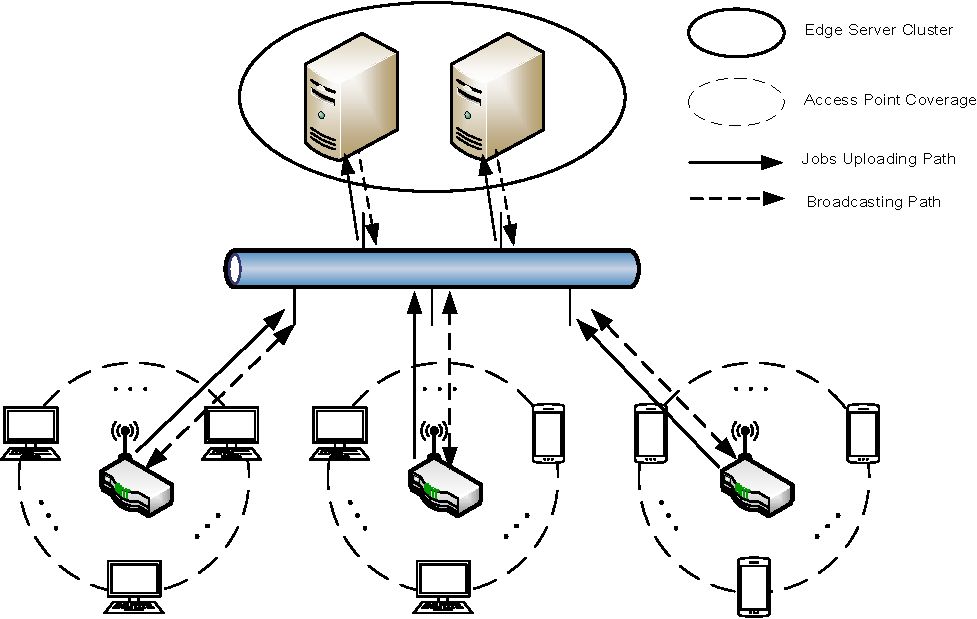
\includegraphics[width=0.45\textwidth, trim={0.5cm 0.5cm 0.5cm 0.5cm}, clip]{system-model.pdf}
                \caption{The Illustration of MEC System Model}
                \label{fig:system}
            \end{figure}

            The offloaded jobs in each timeslot are then immediately dispatched to edge servers which compose the \emph{uploading process} over all AP-ES paired links. We assume that the uploading delay is independent of computation job types and is deterministic for one AP-ES link, which is denoted as $t^{u}_{k,m}$ timeslots from $k$-th AP to $m$-th ES ($\forall k\in\apSet, \forall m\in\esSet$).
            The \emph{parallel uploading} is enabled on AP nodes to alleviate the extra waiting cost caused by serially uploading. As the arrival process and uploading time is bounded, there will be at most $\lambda_k \cdot \max_m(t^{(u)}_{k,m})$ jobs in transmission on $k$-th AP which results into finite bandwidth allocation.
        \end{subsection}

        \begin{subsection}{Information-Sharing Broadcast Model}
            The information sharing is designed with \emph{aligned broadcast} to achieve decentralized cooperation among AP nodes. The \emph{aligned broadcast} is a periodic broadcast mechanism where all the AP and ES nodes start to broadcast at the start of same timeslot, and then repeat broadcasting with the same interval as $t_B$ timeslots. We call each aligned broadcast timeslot as \emph{broadcast point}, which is indexed with $t_i$ for $i$-th broadcast where,
            \begin{align}
                t_i = i \cdot t_B, i=0,1,2\dots
            \end{align}

            After the broadcast point $t_i$, different AP nodes will receive the broadcast information from AP nodes or ES nodes with different deterministic delay.
            Let $d^{(p)}_{k,k'}$ denotes the broadcast delay from $k'$-th AP to $k$-th AP ($\forall k,k'\in\apSet$) w.r.t. the last broadcast point; let $d^{(s)}_{k,m}$ denotes the broadcast delay from $m$-th ES to $k$-th AP ($\forall k\in\apSet,\forall m\in\esSet$). We furthermore call the delay when the AP node could receive all the broadcast information happened at $t_i$ as \emph{consensus delay}, which is defined as following:
            \begin{definition}[Consensus Delay]
                \begin{align}
                    t^{(d)}_k = \max \Paren{\set{d^{(p)}_{k,k'}|\forall k,k'\in\apSet}, \set{d^{(s)}_{k,m}|\forall k\in\apSet,m\in\esSet}},
                \end{align}
                where $d^{(p)}_{k,k} \equiv 0$ for convenience. The consensus delay is the time after last broadcast point where $k$-th AP could obtain the global state view and come to consensus with the complete information.
            \end{definition}
                        
            The broadcast design introduces a \emph{Two-time scale} structure in the MEC system. The job dispatching on AP nodes and scheduling on ES nodes are still carried out based on timeslot scale. However, based on the broadcast period, the uploading process and computing process is separated into consideration.
            More specifically, the uploaded jobs in current broadcast interval will keep waiting on edge servers; at the end of this broadcast interval (just before next broadcast point), the uploading jobs will join the queue on servers for scheduling. This separated process assumption will alleviate the curse of dimensionality in problem formulation, which considers the uploading process not entangled with computation process.
            \hl{Moreover, it's reasonable to assume that the broadcast interval is always larger than any broadcast delay plus the uploading delay for any AP nodes, i.e. $t_B > t^{(d)}_{k} + t^{(u)}_{k,m}$ $(\forall k\in\apSet, \forall m\in\esSet)$.}
            
            At the broadcast point, the AP nodes should broadcast their system information at the broadcast point to the other AP nodes, and the ES nodes should also broadcast their information to all AP nodes. According to the communication model and computation model illustrated above, there would be accumulated jobs which composes the system information on AP and ES nodes respectively.
            More specifically, the information of $i$-th broadcast for $k$-th AP ($\forall k\in\apSet$) contains $\vec{u}_k(i) \define \set{u_{k,m}(i)|\forall m\in\esSet}$, where $u_{k,m}(i)$ denotes the number of unfinished uploading jobs at time $t_i$, i.e. the number of jobs will arrive onto servers in next broadcast interval; the information for $m$-th ES ($\forall m\in\esSet$) contains $Q_m(i)$ to denote the computation queue, where each element $e \in Q_m(i)$ denotes the remaining processing time for that job.
            
            The global system information is composed of all the broadcast information, i.e. the global system states at $t_i$ which is denoted as:
            \begin{align}
                \Obsv_i \define \Brace{ \set{u_{k,m}(i)|\forall k\in\apSet,m\in\esSet}, \set{Q_m(i)|\forall m\in\esSet} },
            \end{align}
            where $\Obsv_i$ is a set of global information of $i$-th aligned broadcast.
        \end{subsection}

        \begin{subsection}{Computation Model}
            For computation process on edge servers, we adopt \emph{unrelated machines} assumption in \cite{tan-online}, where the job processing time on different servers are machine dependent and variant of resource or VM (virtual machine) constraints.
            The maximum processing time in this system is bounded with $L_C$.
            The job space is denoted as $\jSpace$ and its cardinality is denoted as $|\jSpace|=(L_C)^M$ for all possible job processing time on all $M$ ES nodes.
            Moreover, we have the mapping function $f:\jSpace \to \domZ^M$ to store processing time vector for different jobs.
            Additionally, the jobs arrival process on each AP node has the same distribution over job set $\jSpace$ which is denoted as: $p_j \define \Pr(j\in\jSpace)$.
            
            We assume the scheduling policy on all the servers as following:
            \begin{assumption}[Scheduling Policy]
                All the edge servers adopt \emph{FCFS} (First-Come-First-Serve) as job scheduling policy, i.e. the job earlier arrives at the server would get served earlier. And we note that the arrival order is not only determined by job arrives at the access point, but also related with the uploading latency.
            \end{assumption}
        \end{subsection}
    \end{section}

    %============================ FORMULATION =============================%
    \begin{section}{FORMULATION}
        \label{sec:formulation}
        In this section, we formulate the standard MDP problem with respect to the broadcast-point time scale. The formulated problem is based on global information shared via \emph{aligned broadcast}, and the the optimal solution is composed of dispatching policies on all AP nodes. The AP nodes would obtain global states update only after \emph{consensus delay} in each broadcast interval, but they solve the same global optimization problem fully distributed.

        \begin{subsection}{System State and Dispatching Policy}
            The system states is selected based on the nature that $k$-th AP comes to the \emph{global consensus} only after the corresponding \emph{consensus delay} in the broadcast interval.
            The relative difference between broadcast point and global consensus point is depicted in Fig. \ref{fig:br-trans} \hl{(need to modify the state denotation in figure)}. It has to represent the state for AP nodes before and after the consensus point.

            Thus, the system state of the distributed MDP problem based on the global consensus information is given as following:
            \begin{definition}[System State]
                The system state at $i$-th broadcast point is denoted as $\Stat_i \define (\Obsv_{i}, \Obsv_{i-1}), (i=1,2,\dots)$.
                The $k$-th AP nodes would come up with this global state only after $t^{(d)}_k$ timeslots delay w.r.t $t_i$.
            \end{definition}
            \begin{figure}[ht]
                \centering
                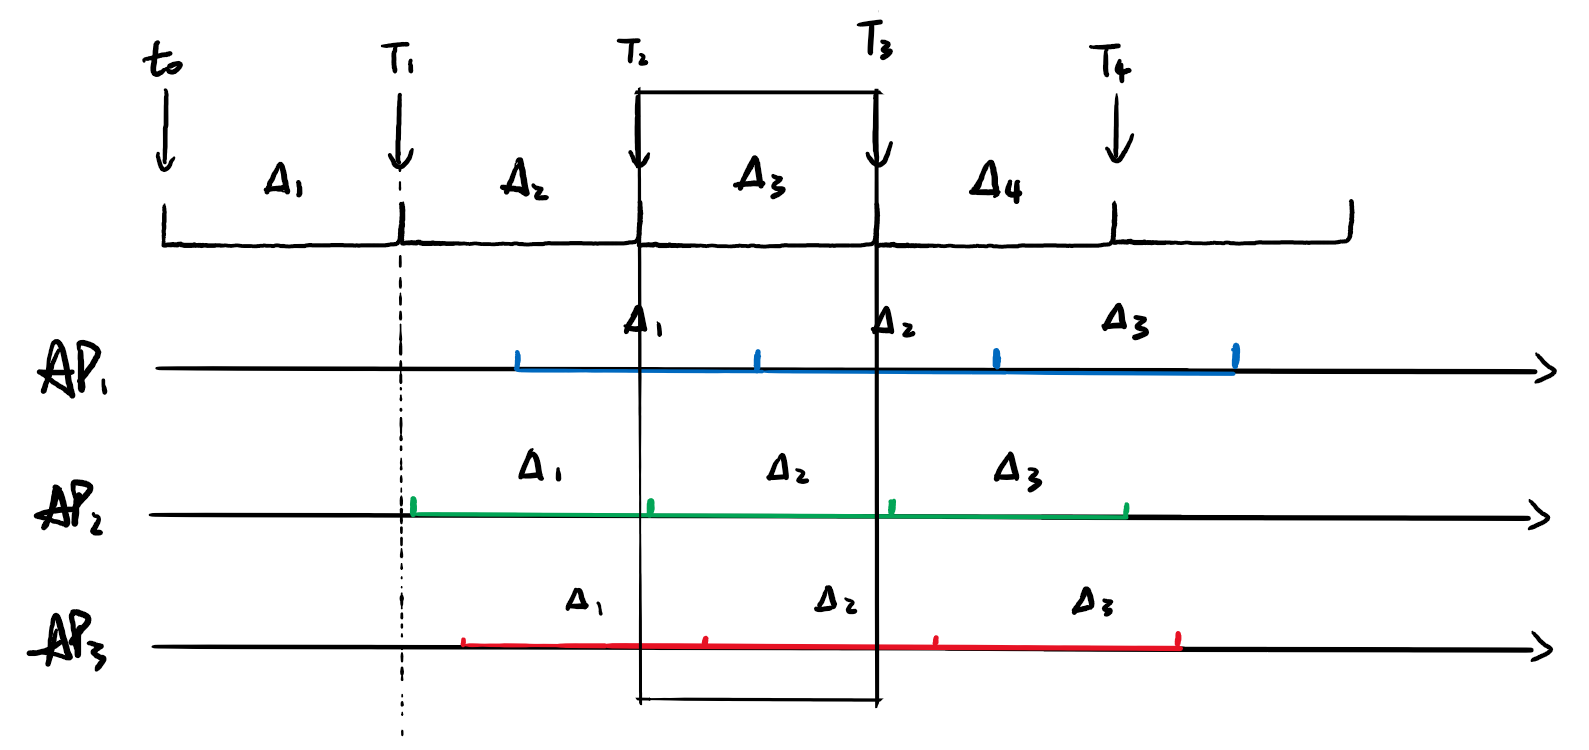
\includegraphics[width=0.45\textwidth]{broadcast-trans.png}
                \caption{Global Consensus and Transition with Delayed Action}
                \label{fig:br-trans}
            \end{figure}

            The \emph{dispatching policy} is applied over arrival jobs in each timeslot on each AP, and the \emph{dispatching action space} is defined as $\vec{a}: (j, m) \in \jSpace \times \esSet$, where $(j, m)$ denotes the action that $j$-type job should be uploaded to $m$-th ES. Based on the two stages of global consensus with obsolete information $\Obsv_{i-1}$ and the updated information $\Obsv_{i}$ in system state, the compounded global-wise policy of all AP nodes is defined as following:
            \begin{definition}[Compounded Dispatching Policy]
                The compounded dispatching policy over $\Stat_{i}$ is defined as $\Policy(\Stat_{i})$ which is composed of all the local policies $\Omega_k(\Stat_{i})$ ($\forall k\in\apSet$) as:
                \begin{align}
                    \vec{\Omega}(\Stat_{i}) \define \Bracket{\Omega_1(\Stat_{i}), \dots, \Omega_K(\Stat_{i})}
                \end{align}
                More specifically, $\Omega_k(\Stat_{i})$ is composed of two-stage policy with $\omega_k(\Obsv_{i-1})$ and $\omega_k(\Obsv_{i})$ as:
                \begin{align}
                    \Omega_k(\Stat_i) = 
                    \begin{cases}
                        \set{\omega^{(i-1)}_{k,m}(j)|\forall m\in\esSet}, & 0 \leq \Delta{t} < t^{(d)}_k
                        \\
                        \set{\omega^{(i)}_{k,m}(j)|\forall m\in\esSet}, & t^{(d)}_k \leq \Delta{t} \leq t_B
                    \end{cases}
                \end{align}
                where $t\in[t_{i-1}, t_{i}], \Delta{t} \define t - t_{i-1}$; $\omega^{(i)}_{k,m}(j)$ denotes the dispatching policy that: based on global information $\Obsv_{i}$, the stochastic action on $k$-th AP upload $j$-type job ($\forall j\in\jSpace$) to $m$-th ES, $\sum_{m\in\esSet}\sum_{j\in\jSpace} \Pr\{\omega^{(i)}_{k,m}(j)\}=1$.
            \end{definition}
        \end{subsection}

        \begin{subsection}{The Optimization Problem}
            The optimization target of our problem is to minimize the \emph{average response time} of all jobs, which is composed of uploading time from AP to ES, and waiting time and service time on ES. According to \emph{Little's Law}, the average response time of all the jobs is equally as average number of jobs in system. Therefore, based on the system state definition, we have cost function as:
            \begin{align}
                g \bigg( \Stat_{i}, \Policy(\Stat_{i-1}) \bigg) \define \sum_{k\in\apSet} \Inorm{\vec{u}_{k}(i)} + \sum_{m\in\esSet} \norm{Q_m(i)},
            \end{align}
            where $\Inorm{\vec{u}_{k}(i)}$ denotes the l1-norm of vector $\vec{u}_{k}(i)$, i.e. the sum up of absolute value of each entry; $\norm{Q_m(i)}$ denotes the number of jobs in queue $Q_m(i)$. The cost function defined is a sampling of interval $t_B$ over the whole process, because the global consensus information for AP nodes only contains the information at the broadcast points.

            Our distributed optimization problem definition is given as following:
            \begin{problem}[Distributed Cooperative Job Dispatching Problem]
                \begin{gather}
                    \min_{\Policy} \lim_{T \to \infty}
                        \mathbb{E}_{\Policy, \{A_k(t)|\forall k\in\apSet\}}
                            \Bracket{\sum_{i=2}^{T} \gamma^{i-1} g(\Stat_{i}, \Policy(\Stat_{i-1}))|\Stat_1},
                \end{gather}
                where the cost is collected with a discount factor $\gamma$.
            \end{problem}

            According to \cite{sutton1998introduction}, the above problem could be solved by the following \emph{Bellman's equation}:
            \begin{align}
                V(\Stat_{i}) =& g(\Stat_i) + \gamma \min_{\Policy(\Stat_{i})} \sum_{\Stat_{i+1}} \Pr\{ \Stat_{i+1}|\Stat_{i}, \Policy(\Stat_{i}) \} V(\Stat_{i+1})
                \nonumber\\
                =& g(\Stat_{i}) + \gamma \min_{\Policy(\Stat_{i})} \sum_{\Stat_{i+1}} \Pr\{ \Stat_{i+1}|\Stat_{i}, \Policy(\Stat_{i}) \}
                    \nonumber\\
                    & \cdot \Bracket{ W^{(p)}\Paren{\Obsv^{(p)}(i+1)} + W^{(s)}\Paren{\Obsv(i+1)} },
            \end{align}
            where $W^{(p)}(\cdot)$ and $W^{(s)}(\cdot)$ denote the split value function over AP nodes and ES nodes respectively; $\Obsv^{(p)}(i) \define \set{\vec{u}_k(i)|\forall k\in\apSet}$ and $\Obsv^{(s)}(i) \define \set{Q_m(i)|\forall m\in\esSet}$ respectively denote the AP states collection and ES states collection for $\Obsv(i) = \set{\Obsv^{(p)}(i), \Obsv^{(s)}(i)}$, and the split value function is in the following form:
            \begin{align}
                W^{(p)}&\Paren{\Obsv^{(p)}(i)} \define \sum_{k\in\apSet}
                    \mathbb{E}_{\Policy}\Bracket{\sum_{n=0}^{\infty} \gamma^{n} \Inorm{\vec{u}_k(i+n)}}
                \\
                W^{(s)}&\Paren{\Obsv(i)} \define \sum_{m\in\esSet}
                    \mathbb{E}_{\Policy}\Bracket{\sum_{n=0}^{\infty} \gamma^{n} |Q_m(i+n)|}
            \end{align}

            \begin{lemma}[Value Function Decoupling]
                According to cost function, the value function could be divided linearly into two section as $ W^{(p)}(\Obsv^{(p)}(i))$ and $W^{(s)}(\Obsv(i))$.
            \end{lemma}
            \begin{proof}
                Please refer to appendix \ref{value-decouple}.
            \end{proof}

            Before diving into analysis on the transition function expression, we firstly come up with some probability denotations.
            % As we separate the uploading process and computation process in the broadcast interval, we take the uploading process as \emph{black box} with only number information contained in state $\vec{u}_k$ ($\forall k\in\apSet$) for all AP nodes.
            The job arrival processes for AP nodes under dispatching policy compose the job arrival process for ES nodes, which could be expressed as compounded of \emph{arrival numbers distribution} and \emph{arrival job-types distribution}.
            \begin{itemize}
                \item
                    The \emph{arrival numbers distribution} on $m$-th ES is composed of i.i.d Bernoulli distribution in each timeslot from $k$-th AP ($\forall k\in\apSet$). The PMF (probability mass function) of the Bernoulli distribution under policy $\omega^{(i)}_{k,m}$ is denoted as:
                    \begin{align}
                        p^{(\lambda,i)}_{k,m} \define \lambda_k \sum_{j\in\jSpace} p(j)
                            \frac{
                                \Pr\{\omega^{(i)}_{k,m}(j)\}
                            }{
                                \sum_{k\in\apSet} \Pr\{\omega^{(i)}_{k,m}(j)\}
                            },
                        % \nonumber\\
                        % \Pr\{\text{one job from $k$-AP to $m$-ES under policy $\omega^{(i)}$}\}
                    \end{align}
                    and we have $p^{(\lambda,\Pi_k)}_{k,m}$ denotes the distribution under time-invariant policy $\Pi_{k}$ for $k$-th AP.
                \item
                    The \emph{arrival job-types distribution} on $m$-th ES from $k$-th AP under policy $\omega^{i}_{k,m}$ is denoted as:
                    \begin{align}
                        p^{(\theta, i)}_{k,m}(j) \define p(j)
                            \frac{
                                \Pr\{\omega^{(i)}_{k,m}(j)\}
                            }{
                                \sum_{k\in\apSet} \Pr\{\omega^{(i)}_{k,m}(j)\}
                            }\;(\forall j\in\jSpace),
                    \end{align}
                    where $p^{(\theta, i)}_{k,m}(j) \geq 0, \sum_{j\in\jSpace}\sum_{m\in\esSet} p^{(\theta, i)}_{k,m}(j)=1$; and we have $p^{(\theta,\Pi_k)}_{k,m}(j)$ denotes the probability under time-invariant policy $\Pi_k$ for $k$-th AP nodes.
            \end{itemize}
            
            \begin{lemma}[Transition Function Decoupling]
                The transition function in Bellman's equation could be decoupled to facilitate the final approximated value function expression. The transition function could be decoupled as:
                \begin{align}
                    & \Pr\{\Stat_{i+1}|\Stat_{i}, \Policy(\Stat_{i})\} 
                    \nonumber\\
                    =& \prod_{k\in\apSet} \Pr\Brace{\vec{u}_k(i+1)|\Policy(\Stat_{i})} \times
                        \nonumber\\
                        & \prod_{m\in\esSet}
                            \Pr \Brace{Q_m(i+1)|Q_m(i), \set{\vec{u}_k(i)|\forall k\in\apSet}, \Policy(\Stat_{i})},
                \end{align}
                where first production part denotes the unfinished uploading state transition for AP nodes whose distribution, and the second part denotes the queueing state transition for ES nodes.
            \end{lemma}
            \begin{proof}
                Please refer to appendix \ref{trans-decouple}.
            \end{proof}

            As the formulated problem above is of infinite states and the action space would be exponentially expanded with respect to number AP and ES nodes, we could not use traditional \emph{policy iteration} or \emph{value iteration} algorithm \cite{sutton1998introduction} for unacceptable computational complexity. To alleviate curse of dimensionality, we take baseline dispatching policy to approximate the value function for each AP and ES nodes, and then carry out one-step iteration to obtain a better value function approximation.
        \end{subsection}
    \end{section}

    %============================= ALGORITHM ==============================%
    \begin{section}{LOW-COMPLEXITY SOLUTION}
        \label{sec:algorithm}
        In this section, we introduce a heuristic dispatching algorithm as the baseline policy, whose value function could be derived analytically. Then the joint expression with transition function as the optimization problem on right-hand side, we could further reduce the state complexity with averaged queueing dynamics on ES nodes.
        \hl{The proposed low-complexity suboptimal policy can be obtained via the above approximated value function and one-step policy iteration. The derived value function becomes the cost upper bound of the proposed policy.}

        \begin{subsection}{Baseline Dispatching Policy}
            The baseline dispatching policy is adopted to obtain an approximation of value function. The policy on each AP nodes is randomized and time-invariant which is denoted as:
            \begin{align}
                \vec{\Pi} \define \Bracket{\Pi_1, \Pi_2, \dots, \Pi_K},
            \end{align}
            where $\Pi_k = \set{\omega_{k,m}|\forall m\in\esSet}$, $\forall k\in\apSet$.

            The decoupled value functions for AP and ES nodes is obtained with an approximated form under the baseline policy.
            
            The approximated value function $\tilde{W}^{(p)}(\Obsv^{(p)}(i+1))$ for AP nodes is obtained as:
            \begin{align}
                \tilde{W}^{(p)}(\Obsv^{(p)}(i+1))
                = \frac{1}{1-\gamma} \sum_{k\in\apSet} \mathbb{E}_{\Pi_k}[\Inorm{\vec{u}_k}],
            \end{align}
            where the expectation of $\Inorm{\vec{u}_k}$ under the policy $\Pi_k$ is actually a constant as expectation of a Binomial distribution as $\mathbb{E}_{\Pi_k}[\Inorm{\vec{u}_k}] = t^{(u)}_{k,m} p^{(\lambda, \Pi_k)}_{k,m}$.
            
            The approximated value function $\tilde{W}^{(s)}(\Obsv(i))$ for ES nodes is affected with both arrival process under dispatching policy and last queue state, and we reduce the states expression by averaging the uploading process together with the transition function expression.
            % For convenience, we have $\Obsv^{(p)}(i) \define \set{\vec{u}_k(i)|\forall k\in\apSet}$ and $\Obsv^{(s)}(i) \define \set{Q_m(i)|\forall m\in\esSet}$.
            The partial value function optimization for ES in Bellman's Equation right-hand side is given as:
            \begin{align}
                \min_{\Policy(\Stat_i)}& \sum_{\Stat_{i+1}}
                    \Pr\Brace{\Stat_{i+1}|\Stat_{i}, \Policy(\Stat_i)} \cdot \tilde{W}^{(s)}\Paren{\Obsv(i+1)}
                \nonumber\\
                % \leadto \min_{\Policy(\Stat_i)}& \sum_{\Obsv^{(s)}(i)} \Pr\{\Obsv^{(s)}(i+1)|\Obsv^{(s)}(i),\Obsv^{(p)}(i), \Policy(\Stat_i)\}
                %     \nonumber\\
                %     & \times \sum_{\Obsv^{(p)}(i)} \Pr\{\Obsv^{(p)}(i+1)|\Policy(\Stat_i)\} \cdot \tilde{W}^{(s)}(\Obsv(i+1))
                % \nonumber\\
                \leadto \min_{\Policy(\Stat_i)}& \sum_{\Obsv^{(s)}(i)}
                    \Pr\Brace{\Obsv^{(s)}(i+1)|\Obsv^{(s)}(i), \Obsv^{(p)}(i), \Policy(\Stat_i)}
                    \nonumber\\
                    & \times \sum_{m\in\esSet}
                        \mathbb{E}_{\Obsv^{(p)}(i+1)|\Policy(\Stat_i)}\Bracket{\tilde{W}^{(s)}_m\Paren{\Obsv(i+1)}}
            \end{align}
            Let $\tilde{V}^{\Policy(\Stat_i)}(Q_m(i+1)) \define \mathbb{E}_{\Obsv^{(p)}(t+1)|\Policy(\Stat_t)} [\tilde{W}^{(s)}_m(\Obsv(i+1))]$ denotes the averaged value function for $m$-th ES node, which implies that the state $\Obsv^{(p)}(i)$ is substitute with its expectation under policy $\Policy(\Stat_i)$ in this value function.

            Furthermore, the approximated value function could be rewrite with reduced states for stationary FCFS process as $\tilde{V}^{\Policy(\Stat_i)}(\tilde{Q}_m(i+1))$, where $\tilde{Q}_m(i+1) \define [N_m(i+1), r_m(i+1)]$, $N_m(i+1)$ denotes the number of jobs in $m$-th queue and $r_m(i+1)$ denotes the remaining time of last unfinished job. Thus the approximated value function for $m$-th ES node is denoted as:
            \begin{align}
                \tilde{V}\bigg(\tilde{Q}_m(i+1)\bigg) \define& \lim_{T\to\infty}
                    \mathbb{E}_{\vec{\Pi}} \Bracket{\sum_{n=0}^{T} \gamma^{n} N_m(i+1)}
                \nonumber\\
                % =& \vec{u}'_i [\lim_{T\to\infty} \sum_{n=0}^{T} (\gamma \mat{P}_m)^{n}] \vec{g}_q
                % \nonumber\\
                =& \vec{u}'_i \Paren{\mat{I} - \gamma \mat{P}_m}^{-1} \vec{g}_q,
            \end{align}
            where $\vec{\mu}'_i$ denotes the transpose of $\vec{\mu}_i$, and $\vec{\mu}_i = [0,\dots,0,1,\dots]$ with only $i$-th element as $1$; the $i$-th element of $\vec{g}_q$ denotes the cost of server as $N_m(i)$ for $i$-th stage; $\mat{P}_m$ denotes the transition matrix under the policy $\vec{\Pi}$ which is composed of the following transition function ($\forall \tilde{Q}_m(i),\tilde{Q}_m(i+1)$) as:
            \begin{align}
                & \Pr \Brace{\tilde{Q}_m(i+1)|\tilde{Q}_m(i),\vec{\Pi}}
                \nonumber\\
                % =& \Pr\{\begin{pmatrix}
                %     N_m(i+1) \\ r_m(i+1)
                % \end{pmatrix}|\begin{pmatrix}
                %     \tilde{N}_m(i+1) \\ r_m(i)
                % \end{pmatrix}\}
                % \nonumber\\
                =& \prod_{k\in\apSet} \Pr\{\tilde{N}^{(k)}_m(i)\} \prod_{n=0}^{\tilde{n}_0 + \tilde{N}^{(k)}_m(i)} p^{(\theta,\Pi_k)}_{k,m}(j_{k,n})
                    \nonumber\\
                    &\times I[\tilde{N}^{(k)}_m(i) = N^{(k)}_m(i+1)- \tilde{n}_0]
                    \nonumber\\
                    &\times I[\sum_{j_{k,n}} f(j_{k,n})^{(m)} = r_m(i+1)+t_B-r_m(i)],
            \end{align}
            where:
            \begin{itemize}
                \item $f:\jSpace \to \domZ^M$ is the mapping function from job-type index to job processing time vector of all servers, and $f(j)^{(m)}$ denotes the $m$-th entry of $j$-type job;
                \item $\tilde{n}_0 = t^{(u)}_{k,m}p^{(\lambda,i)}_{k,m}$ is the averaged $\Obsv^{(AP)}$ state under policy $\Policy(\Stat_i)$;
                \item $\tilde{N}^{(k)}_m(i) \sim Bin(t_B-t^{(u)}_{k,m}, p^{(\lambda, \Pi_k)}_{k,m}), (\forall k\in\apSet)$.
            \end{itemize}
        \end{subsection}

        \begin{subsection}{The Distributed Algorithm}
            The approximate Bellman's equation under baseline policy is denoted as:
            \begin{align}
                % V(\Stat_i) = &g(\Stat_i) +
                % \nonumber\\
                \min_{\Policy(\Stat_i)}& \sum_{\Obsv^{(s)}(i+1)} \Pr\{\Obsv^{(s)}(i+1)|\Obsv^{(s)}(i), \Obsv^{(p)}(i), \Policy(\Stat_i)\}
                \nonumber\\
                \times \bigg[& \sum_{m\in\esSet} \tilde{V}^{\Policy(\Stat_i)}\bigg(\tilde{Q}_m(i+1)\bigg) +
                    \nonumber\\
                    & \underbrace{\sum_{\Obsv^{(p)}(i+1)} \Pr\{\Obsv^{(p)}(i+1)|\Policy(\Stat_i)\}}_{\text{Expectation of Binomial}|\Policy(\Stat_i)}
                    \cdot \underbrace{\tilde{W}^{(p)}\bigg(\Obsv^{(p)}(i+1)\bigg)}_{\text{constant}} \bigg]
            \end{align}
            Then we introduce the one-step iteration algorithm:
            % [\IF, \ENDIF], [\FOR, \TO, \ENDFOR], [\WHILE, \ENDWHILE], \STATE, \AND, \TRUE
            \begin{algorithm}[H]
                \caption{Distributed Algorithm for $k$-th AP}
                \begin{algorithmic}
                    \WHILE{\TRUE}
                        \STATE (in progress ...)
                        % \FOR{$k \in \mathcal{K}$}
                        %     \STATE fix policy $\vec{\Omega}^{(k)}(t) \forall k' \neq k$
                        % \ENDFOR
                    \ENDWHILE
                \end{algorithmic}
            \end{algorithm}
        \end{subsection}
        
    \end{section}

    %============================ EVALUATION ==============================%
    \begin{section}{EVALUATION}
        \label{sec:evaluation}
        (in progress ...)
    \end{section}

    %============================= CONCLUSION =============================%
    \begin{section}{CONCLUTION}
        \label{sec:conclusion}
        (in progress ...)
    \end{section}
    
    %============================== APPENDIX ==============================%
    \appendices

    \begin{section}{Value Function Decoupling}
        \label{value-decouple}
        \begin{align*}
            V(\Stat_i) \define& \mathbb{E}_{\Policy} \Bracket{\sum_{n=0}^{\infty} \gamma^{n} g\Paren{\Stat_{i+n},\Policy(\Stat_{i+n-1})}}
            \nonumber\\
            =& \mathbb{E}_{\Policy} \Bracket{\sum_{n=0}^{\infty} \gamma^{n} \sum_{k\in\apSet} \Inorm{\vec{u}_{k}(i)} + \sum_{m\in\esSet} \norm{Q_m(i)}}
            \nonumber\\
            =& \sum_{k\in\apSet} \mathbb{E}_{\Policy}\Bracket{\sum_{n=0}^{\infty} \gamma^{n} \Inorm{\vec{u}_k(i+n)}} 
                \nonumber\\
                &+\sum_{m\in\esSet} \mathbb{E}_{\Policy}\Bracket{\sum_{n=0}^{\infty} \gamma^{n} |Q_m(i+n)|}
            \nonumber\\
            =& W^{(p)}\Paren{\Obsv^{(p)}(i)} + W^{(s)}\Paren{\Obsv(i)}
        \end{align*}
    \end{section}

    \begin{section}{Transition Function Decoupling}
        \label{trans-decouple}

        The first production part is given as:
        \begin{align*}
            \Pr\{\vec{u}_k=\vec{u}|\Policy(\Stat_i)\} \sim \prod_{m\in\esSet}
                Bin\Paren{t^{(u)}_{k,m}-1,p^{(\lambda, i)}_{k,m}},
        \end{align*}
        where $Bin(n,p)$ denotes a Binomial distribution.
            
        The second part transition function is rather complex and composed of three independent distribution as depicted in Fig. \hl{(need a timeline graph)}. We denote the state $Q_m(i+1)$ over the three stages as:
        \begin{align*}
            Q_m(i+1) = [\tilde{Q}_m(i), Y_0, Y_1, Y_2],
        \end{align*}
        where $\tilde{Q}_m(i)$ denotes the remaining part of the previous $Q_m(i)$ after $t_B$ timeslots computing in $[t_{i}, t_{i+1}]$, and:
        \begin{itemize}
            \item $Y_0$ denotes the enqueued job set from unfinished uploading jobs in last interval as $\set{u_{k,m}(i)|\forall k\in\apSet}$, where $n^{(k)}_0 \define u_{k,m}(i)$, $|Y_0|=\sum_{k\in\apSet} u_{k,m}(i)$;
            \item $Y_1$ and $Y_2$ respectively denotes the enqueued job set uploaded by all AP nodes under policy $\omega_{k,m}^{i-1}$ and $\omega_{k,m}^{i}$, where $|Y_1|\define\sum_{k\in\apSet}N^{(k)}_1, |Y_2|\define\sum_{k\in\apSet}N^{(k)}_2$.
        \end{itemize}
        Then we have the transition function for $m$-th ES node given as:
        \begin{align*}
            & \Pr\Brace{Q_m(i+1)|Q_m(i), \set{\vec{u}_k(i)|\forall k\in\apSet}, \Policy(\Stat_i)}
            \nonumber\\
            =& \Pr\Brace{\tilde{Q}_m(i)|Q_m(i)}
                \Pr\Brace{Y_0, Y_1, Y_2|\set{\vec{u}_k(i)|\forall k\in\apSet}, \Policy(\Stat_i)}
            \nonumber\\
            =& \prod_{k\in\apSet} \Pr\Brace{N^{(k)}_1,N^{(k)}_2}
                \Bracket{
                    \prod_{n=1}^{n^{(k)}_0 + N^{(k)}_1} p^{(\theta, i-1)}_{k,m}(j_n)
                }
                \Bracket{
                    \prod_{n=1}^{N^{(k)}_2} p^{(\theta, i)}_{k,m}(j_n)
                }
        \end{align*}
        where $N^{(k)}_1$ and $N^{(k)}_2$ are independent and follow two different Binomial distributions respectively as:
        \begin{align*}
            N^{(k)}_1 &\sim Bin\Paren{t^{(d)}_k, p^{(\lambda, i-1)}_{k,m}}
            \\
            N^{(k)}_2 &\sim Bin\Paren{t_B-t^{(d)}_k-t^{(u)}_{k,m}, p^{(\lambda, i)}_{k,m}}
        \end{align*}
    \end{section}
    
    %============================== REFERENCE =============================%
    \bibliographystyle{IEEEtran}
    \bibliography{main.bib,journal-ref.bib}
\end{document}